%!TEX root = ../template.tex
%%%%%%%%%%%%%%%%%%%%%%%%%%%%%%%%%%%%%%%%%%%%%%%%%%%%%%%%%%%%%%%%%%%%
%% chapter2.tex
%% NOVA thesis document file
%%
%% Chapter with the template manual
%%%%%%%%%%%%%%%%%%%%%%%%%%%%%%%%%%%%%%%%%%%%%%%%%%%%%%%%%%%%%%%%%%%%

\typeout{NT FILE demmon.tex}

\chapter{DeMMON}
\label{cha:demmon}
\input{Chapters/pseudocode/jlt-pseudocode.tex}

DeMMon (Decentralized Management and Monitoring Overlay Network) is an overlay network aiming to create logical connections among nodes integrating the network, forming multiple tree-shaped networks. Then, it provides an API to request information about nodes and services running in the system, which is collected on-demand by the monitoring protocol via efficient information aggregation and dissemination using the tree structure.

In this chapter, we will begin by explaining the targeted environment and the operation of the overlay network, whose tree shape is the basis for the aggregation protocol. After, detail how the aggregation protocol performs aggregations in the tree, and lastly, list the operations exposed by the API and discuss how it interacts with the remaining components. \todo{insert refs to subsections ahead}

This solution, as observable in figure \ref{fig:demmon-overview}, is composed of three major components:

\begin{figure}[htbp]
    \centering
    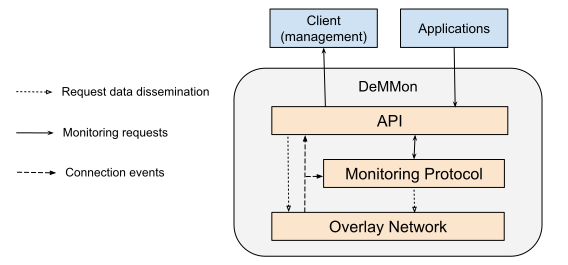
\includegraphics[width=\textwidth]{Chapters/Figures/DeMMon-arch-overview.pdf}
    \caption{An overview of the architecture of DeMMon}
    \label{fig:demmon-overview}
\end{figure}


\begin{enumerate}
    \item The overlay network, which strives to build the tree-shaped network, nodes in this network use proximity and a set of logical rules to change their location in the tree.

    \item The monitoring protocol, which is a component that collects and disseminates information using the overlay network's established connections. It communicates via notifications and asynchronous request-replies with the overlay network to receive updates regarding established connections and connection failures. Lastly, it receives requests from the API to collect information.

    \item Lastly, the API receives updates from both the overlay network and the monitoring protocol, exposes the received information from those layers, and allows ingestion of new information. Furthermore, it allows issuing commands to collect new information, perform local aggregations periodically, or trigger issued alarms based on the respective conditions.
\end{enumerate}

\section{Overlay network}

In this section, we discuss the design of the overlay network, which aims to build and maintain a latency and bandwidth aware tree-shaped network. We begin by providing the considered system model, then follow with an overview of the mechanisms responsible for building and maintaining the tree. Lastly, we conclude the chapter with a summary and discussion of the protocol.

\subsection{System Model}

The assumed system model is assumed to be a distributed scenario composed of nodes connected to the internet set-up such that they can send and receive messages via the internet (i.e. with an external IP or port-forwarding). We also assume that nodes are inserted in an cloud-edge environment, with nodes possibly spread throughout multiple continents and with varied bandwidth values. All nodes run the same software stack with similar configuration settings, installed a priori.

It is assumed that all but a small portion of nodes (also known as the landmarks) can fail, and that nodes that fail do so in a crash-fault manner, stopping the emition and reception of messages. The aforementioned landmarks are representative of nodes running in cloud environments, and consequently, may have increased fault-tolerance using replication.

\subsection{Overview}

The devised protocol

The devised membership protocol is coalesced by four main mechanisms: (1) the \textbf{join} mechanism, which aims to establish the initial tree structure, (2) the \textbf{active view maintenance}, responsible for periodically sharing some information with the parent, and using that information for tree management, (3) \textbf{passive view maintenance}, responsible for collecting information about peers which are not in the active view, used for fault tolerance and for optimizing the tree, and finally, (4) \textbf{fault tolerance}.

\subsubsection{Join mechanism}

As previously mentioned, the join mechanism is the mechanism responsible for creating the initial tree structure, it is the first mechanism to be executed by each node in the system,

% JOIN -----

\begin{algorithm}
    % \setstretch{0.85}
\begin{algorithmic}[1]
    \caption{Join Protocol (Types and state)} \label{alg:state:join}
    \asdtypes
        \State Node \{
        \Indent
            \State lat \Comment{ the measured latency to the peer}
            \State parentIP \Comment{ the IP of the parent of the Node}
            \State nrChildren \Comment{ the number of children}
            \State replied \Comment{ wether the node replied to joinMessage}
            \State IP \Comment{ the node IP}
            \State children: []<IP, nrChildren> \Comment{ the node's children, can be null for certain nodes (i.e. siblings and node's children), and is not sent in messages }
        \EndIndent
    \asdend
    \asdstate \label{alg:state:state}
        \State contactedNodes \Comment{ collection of all successfully contacted nodes}
        \State nodesToContact \Comment{ nodes being contacted}
        \State joinTimeouts \Comment{ collection of contacted nodes -> timerIDs}
        \State bestPeerLastLevel : Node \Comment{the best peer contacted so far in the join process}
        \State joinTimeoutTimerID \Comment{ timerID for join messages}
        \State self : Node \Comment{ myself}
    \asdend
    
\end{algorithmic}
\end{algorithm}


\begin{algorithm}
    % \setstretch{0.85}
\caption{Membership protocol (Join)}
\begin{algorithmic}[1]


\asdupon[Init(landmarks : map{IP}:Node, selfIP, isLandmark)] \label{alg:memb:join:init}
    \State joinTimeouts \asdassign \{\}
    \State prevBestP \asdassign \{\}
    \State landmarks \asdassign [landmarks]
    \IfThenElse{isLandmark}{addSibling(landmarks)}{contactNodes(landmarks)}
\asdend

\asdprocedure[contactNodes(nodeIPs)]
    \State nodesToContact \asdassign \{\}
    \For{p in nodeIPs}
        \State nodesToContact[p] = Node \{IP: p, replied:false,measured: false\}
        \State MeasureNode(p) 
        \State sendMessageSideChannel(JoinMessage<>, p)
        \State joinTimeouts[p] = \asdassign setupTimer(JoinTimeoutTimer(p))
    \EndFor
\asdend

\asdupon[JoinTimeoutTimer(node) || NodeMeasuringFailed(node)]
        \IfThenElse{(L in Landmarks)}{rejoinLater()}{delete(nodesToContact[L])}
    \asdend

\asdupon[receive(Join<>,sender)]
    \State sendMessageSideChannel(JoinReply<self.parent, self.node, self.children>, sender)
\asdend
    
\asdupon[receive JoinReply(<parentIP, node, children>, sender) \&\& \textbf{measuredLatency}(lat)]
        \If{\asdnotin{parentIP}{contactedNodes}}
            \State nodesToContact.delete(node)
        \Else
            \State nodesToContact[node].lat = lat
            \State nodesToContact[node.IP].children \asdassign children
            \State nodesToContact[node.IP].parent \asdassign parentIP
            \State nodesToContact[node.IP].replied \asdassign true
            \State cancelTimer(joinTimeouts[sender])
            \State delete(joinTimeouts, sender)
        \EndIf
\asdend

\asdupon[(forall n $\in$ nodesToContact -> n.replied)]
    \If{ len(nodesToContact) == 0}
    % \Comment{has not gotten past landmarks}
        \IfThenElse{prevBestP == nil}
        {rejoinLater()}
        {joinAsChild(prevBestP) }
        \State return
    \EndIf
    \State contactedNodes.appendAll(nodesToContact)
    \For{node in sortedByLatency(nodesToContact)}
        \If{prevBestP != nil \&\& prevBestP.lat $\le$ node.lat} 
            \State joinAsChild(prevBestP)
            \State return
        \EndIf
        \If{(\asdnotin{node.IP}{landmarks}) \&\& node.nrChildren == 0}
            \State continue \Comment{check if node has enough children}
        \EndIf
        \State prevBestP = node
        \State toContact \asdassign [c -> c.nrChildren >= config.minGroupSize]
        \State contactNodes(toContact)
        \State return
    \EndFor

    \If{prevBestP.parentIP == nil} \Comment{No nodes were suitable, fallback to parent of best previous node}
        \State prevBestP = contactedNodes[prevBestP.parentIP]
        \State joinAsChild(prevBestP)       
        \State return
    \Else
        \State rejoinLater()
        \State return
    \EndIf
\asdend

\asdprocedure[joinAsChild(p : Node)]
    \State joinTimeoutTimerID = setupTimer(JoinRequestTimeout<p>)
    \State sendMessageSideChannel(JoinRequest<>, p.IP)
\asdend

\asdupon[JoinRequestTimeout(p : Node)]
    \If{p.parentIP != nil}
        \State prevBestP = contactedNodes[prevBestP.parentIP]
        \State joinAsChild(prevBestP)
    \Else
        \State rejoinLater()
    \EndIf
\asdend

\asdupon[receive(JoinRequest<>, sender)]
    \State addChildren(sender) \Comment{new chilren is established}
    \State sendMessageSideChannel(JoinRequestReply<generatedID,self,children>, p.IP)
\asdend
    
\asdupon[receive(JoinRequestReply<attributedId,parent,siblings>, sender)]
    \State addParent(sender) \Comment{Parent is established, join complete}
    \State cancelTimer(joinTimeoutTimerID)
\asdend
\end{algorithmic}
\end{algorithm}


\begin{algorithm}
    % \setstretch{0.85}
    \begin{algorithmic}[1]

        \caption{Membership protocol (Active view Optimization)}

        \asdstate
            \State parent \Comment{defined in join}
            \State children 
            \State childrenLatencies : dict<string:dict<string:number>>
        \asdend

        \asdrepeateveryx{config.updatePeriodicity}
            \If{parent != nil}
                \State sLatencies \asdassign set()
                \For{sibling in siblings}
                    \State sLatencies.append(<sibling.IP,sibling.measuredLatency)
                \EndFor
                \State sendMessage(UpdateChildStatus<children, siblingLatencies>, parent)
            \EndIf
            \For{child in chidren}
                \State sendMessage(UpdateParentStatus<self,child.ID, parent>)
            \EndFor
        \asdend

        \asdupon[receive(UpdateParentStatus<parent,myID, grandParent>, sender)]
            \If{sender == parent.IP}
                \State parent \asdassign parent
                \State self.ID \asdassign parent.ID + myID
                \State grandParent \asdassign grandParent
            \EndIf
        \asdend

        \asdupon[receive(UpdateChildStatus<child, childSiblingLatencies>, sender)]
            \If{children[sender] != nil}
                \State childrenLatencies[sender]=childSiblingLatencies
            \EndIf
        \asdend

        \asdrepeateveryx{config.updateChildPeriodicity}
            \State childrenLatValues \asdassign set()
            \For{c1 in children}
                \For{<c2, lat> in childrenLatencies[c]}
                    \If{lat - c1.measuredLatency >= d.config.maxLatDowngrade}
                        e break
                    \EndIf
                    \State higherBwC \asdassign c1
                    \State lowerBWC \asdassign c2
                    \If{c2.bw > c1.bw}
                        \State higherBwC \asdassign c2
                        \State lowerBWC \asdassign c1
                    \EndIf
                    \State childrenLatValues.add(<higherBwC,lowerBWC,lat>)
                \EndFor
            \EndFor
            \State kickedNodes, newParents \asdassign set(),set()
            \State potentialChildren \asdassign dict<string,set<Node{>}{>}
            \State sortByLatency(childrenLatValues)

            \For{<higherBwC,lowerBWC,lat> in childrenLatValues}
                \If{len(children) - len(kickedNodes) <= config.MinGroupSize}
                    \State break
                \EndIf
                \If{higherBwC in kickedNodes or lowerBWC in kickedNodes}
                    \State continue
                \EndIf
                \If{loserBWC in newParents}
                    \State continue
                \EndIf
                \If{higherBwNode.nrChildren == 0}
                    \State potentialChildren[higherBwNode].append(lowerBWC)
                    \If{len(potentialChildren) >= config.MinGroupSize}
                        \For{potentialChild in potentialChildren[higherBwNode]}
                            \State newParents <- newParents + higherBwNode
                            \State send(OptimizationPropose<higherBwNode>, potentialChild)
                            \State higherBwNode.nrChildren++
                            \State kickedNodes <- kickedNodes + potentialChild
                        \EndFor
                        \For{<nIP,pontentialChildrenTmp> in potentialChildren}
                            \State pontentialChildrenTmp.deleteAll(potentialChildren[higherBwNode])
                        \EndFor
                        \State potentialChildren[higherBwNode] \asdassign set<Node>
                        \State continue
                    \EndIf
                \EndIf
                \State kickedNodes <- kickedNodes + lowerBWC
                \State send(OptimizationPropose<higherBwNode>, lowerBWNode)
            \EndFor
        \asdend

        \asdupon[receive(OptimizationPropose<newParent>, sender)]
            \If{sender == parent}
                \State send(OptimizationProposeRequest<sender>, newParent)
            \EndIf
        \asdend

        \asdupon[receive(OptimizationProposeRequest<p>, sender)]
            \If{ p == parent \&\& sender in siblings} \Comment{ parent issuing the message is the same parent that i have}
                \State send(OptimizationProposeRequestReply<true>, sender)
            \Else
                \State sendSideChannel(OptimizationProposeRequestReply<false>, sender)
            \EndIf
        \asdend

        \asdupon[receive(OptimizationProposeRequestReply<reply>, sender)]
            \If{reply}
                \State sendMessageAndDisconnectFrom(DisconnectMessage<>, parent)
                \State addParent(sender)
            \EndIf
        \asdend

    \end{algorithmic}
\end{algorithm}

\begin{algorithm}[H]
\begin{algorithmic}[1]
    
    \caption{Oportunistic Optimization}

    \asdstate
        \State eView : set<Node>
    \asdend

    \asdrepeateveryx{config.RandWalkPeriodicity}
        \State ascNeighs, allNeighs = set
        \State ascNeighs = ascNeighs + parent + siblings
        \State allNeighs = allNeighs + ascNeighs + children
        \State sample = getRandSample(eView + allNeighs, config.NrPeersToMergeRandWalk)
        \State sendMessage(RandomWalk<sample, config.RandWalkTTL, self.ID, self.IP>, getRand(ascNeighs))
    \asdend

    \asdrepeateveryx{config.OportunisticOptimizationTimeout}
        \State toMeasureRand = getRandSample(eView, config.NrPeersToMeasureRandom)
        \State toMeasureBiasedOpts = sortByEuclideanDist(eView / toMeasureRand)
        \State toMeasureBiased = getRandSample(toMeasureBiasedOpts, config.NrPeersToMeasureRandom)
        \For p in toMeasureRand:
            \State measurePeer(p)
        \EndFor
        \For p in toMeasureBiased:
            \State measurePeer(p)
        \EndFor
    \asdend


    \asdupon[receive( RandomWalk<sample, ttl, nID, orig>, sender)]
        \State stepsTaken = config.RandWalkTTL - ttl
        \State nrToAdd = config.NrPeersToMergeRandWalk
        \State nrToMerge = config.NrPeersToMergeRandWalk
        \State ascNeighs, allNeighs = set(), set()
        \State ascNeighs = ascNeighs + parent + siblings
        \State allNeighs = allNeighs + ascNeighs + children

        \If{stepsTaken < config.NrStepsToIgnore}:
            \State nrToMerge = 0
        \EndIf

        \State toAdd = getRandSample(excludeDescendantsOf([eView + allNeighs] / sample),nID), nrToAdd)
        \State toRemoveFromSample = getRandSample(sample, nrToMerge)
        \State sample = sample / toRemoveFromSample
        \State sample = sample + toAdd
        \State target = getRand(excludeDescendantsOf(allNeighs, nID)
        \If{target == nil || ttl == 0}
            \State sendMessageSideChannel(RandomWalkReply<sample>, orig)
        \Else
            \State sendMessage(RandomWalk<sample, ttl-1, nID, orig>, getRandom(ascNeighs))
        \EndIf
        \State eView = excludeDescendantsOf(toRemoveFromSample, self.ID)  + eView
        \State eView = eView / allNeighs
        \State eView = eView[:config.MaxEViewSize]
    \asdend

    \asdupon[peerMeasured(p, latency)]
        \State latencyImprovement := parent.measuredLatency - Latency
        \If{latencyImprovement >= config.MinLatencyForImprovement}
            \State sendMessageSideChannel(OportunisticImprovementReq<self>,p)
        \EndIf
    \asdend


    \asdupon[receive(OportunisticImprovementReq<p>,sender)]
        \If{isDescendent(p.ID,self) or parent == nil}
            \State sendMessageSideChannel(OportunisticImprovementReqReply<false>,sender)
        \Else
            \State addChildren(sender)
            \State sendMessageSideChannel(OportunisticImprovementReqReply<true>,sender)
        \EndIf
    \asdend

    \asdupon[receive(OportunisticImprovementReqReply<answer>,sender)]
        \If {answer} 
            \State addParent(sender)
        \EndIf
    \asdend

    \Function{isDescendentOf}{nodeID, PotentialDescID}
        \State return PotentialDescID.Contains(nodeID)
    \EndFunction

\end{algorithmic}
\end{algorithm}

\subsection{Summary}

\section{Monitoring protocol}

\subsection{Overview}

\subsection{Aggregation mechanisms}

\subsubsection{Single root aggregation}

\subsubsection{Multi root aggregation}

\subsubsection{Neighborhood aggregation}

\subsection{Summary}

\section{API}

\subsection{System Model}

\subsection{Overview}

\subsection{Showcase}